\chapter{Desenvolvimento} \label{desenv}
\pagestyle{simple} 

Nessa seção serão descritas de forma mais detalhada as etapas de análise dos datasets e os processos realizados em cada etapa, visando descrever como as recomendações foram obtidas através do uso das ferramentas e técnicas descritas nas seções anteriores.

\section{Escolha do dataset} \label{escolha-ds}

Para o trabalho foram escolhidos 3 \textit{datasets} de \textit{e-commerce} entre dezenas disponíveis nos repositórios Kaggle e UCI ML. Estes conjuntos foram escolhidos pois possuem características que favorecem sua utilização para testes de sistemas de recomendação, tais como:

\begin{itemize}
    \item Estão disponíveis de forma integral, pública e gratuita
    \item Possuem mais de 100 mil registros
    \item Embora os clientes estejam anonimizados, os conjuntos mantém dados que permitem categorizá-los (ex.: cidade/estado/país de origem)
    \item Os datasets provenientes do UCI ML já foram utilizados com propósitos acadêmicos por \citedir{chen10}
    \item O dataset proveniente do Kaggle recebeu boas avaliações: possui classificação "Ouro" pela plataforma, ganhou 1023 votos positivos de usuários e "Usabilidade" avaliada como nota 10/10. \footnote{Dados referentes ao dia 19/09/2020}
\end{itemize}

\begin{table}[ht]
\centering
\begin{tabular}{@{}lllll@{}}
\toprule
\textbf{Nome}        & \textbf{Nº de registros} & \textbf{Tamanho (MB)} & \textbf{Período} & \textbf{Origem} \\ \midrule
Online Retail        & 541.909                  & 43,4                  & 2010-2011        & UCI ML             \\
Online Retail II     & 1.067.371                & 85,7                  & 2009-2011        & UCI ML            \\
Brazilian E-Commerce & 112.650                   & 7,5                  & 2016-2018        & Kaggle          \\ \bottomrule
\end{tabular}
\caption{Dados sobre os datasets selecionados para o trabalho}
\label{tab:my-table}
\end{table}

\section{Estudo de sistemas de recomendação} \label{estudo-sist}
Decidiu-se por seguir um modelo de filtragem colaborativa, que tal como descrito na Seção \ref{sist-rec} leva em conta apenas as avaliações dadas pelos clientes a um determinado produto e não dados do produto em si. Contudo, há diferentes maneiras de implementar sistemas de desse tipo e portanto antes de iniciar-se o desenvolvimento foi realizada uma busca por tutoriais e projetos de exemplo na Internet que explicassem mais detalhadamente essas implementações. 

Em um dos projetos encontrados, \citedir{tanner18} explica em vídeo uma abordagem semelhante na qual ele treina e testa um modelo de sugestão de livros baseado em avaliações (notas de 1 a 5) das pessoas que os compraram. A rede criada por ele é treinada de forma a aprender a relação entre essas entradas categóricas e suas respectivas saídas, as avaliações, como exemplificado na figura \ref{fig:tanner}.

Nesse trabalho, optou-se por seguir a implementação de Tanner, visto que esta apresenta várias vantagens do ponto de vista de desempenho e manutenção de código que serão explicadas em mais detalhes na Seção \ref{geracao-rec}.

\begin{figure}[htp]
    \centering
    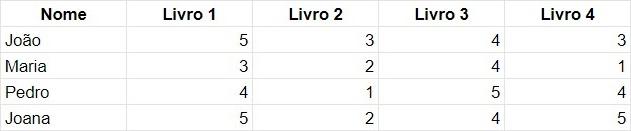
\includegraphics[width=12cm]{doc/latex/text/images/tanner.jpg}
    \caption{Exemplo do sistema de recomendação de Tanner}
    \label{fig:tanner}
\end{figure}

\section{Definição de critério de avaliação} \label{definicao-crit}
Para que se possa utilizar a abordagem ilustrada por \citedir{tanner18} com qualquer \textit{datasets}, é necessário que avaliações numéricas (por exemplo, notas de 1 a 5) estejam relacionadas às transações analisadas. Contudo, não é todo \textit{dataset} que possui esse tipo de dado. Os conjuntos listados na Seção \ref{escolha-ds}, por exemplo, elencam somente pares de clientes/produtos, e portanto o único dado que pode ser inferido desses \textit{datasets} é a frequência de compra por cliente. Visto que não há informação detalhada sobre o produto, abordagens baseadas em conteúdo (características do produto) ou objetivos (para quê o produto serve) não são viáveis.

Foram portanto definidos 3 métodos de criar avaliações para os registros nesses \textit{datasets}, baseados na frequência de compra em diferentes agrupamentos de clientes. Quanto mais popular um produto é, mais passível de recomendação ele se torna. As regras de avaliação foram baseadas nas definições para filtragem colaborativa (FC) no contexto de sistemas de recomendação. 

\begin{itemize}
   \item FC por Categoria: se o cliente não comprou e o produto é popular dentro da categoria na qual o cliente está, define avaliação alta. Isso aumenta a probabilidade de recomendação para produtos populares na categoria (Figura \ref{fig:fc-categ}).
    \item FC Intercategorias: se o cliente em questão não comprou o produto e este é popular dentro da categoria do cliente, define avaliação alta. Se o cliente não comprou, o produto não é popular, mas outro cliente da mesma categoria comprou, define avaliação média. Isso aumenta a probabilidade de recomendação para produtos populares na categoria enquanto também destaca produtos menos populares adquiridos por clientes similares. (Figura \ref{fig:fc-intercateg}).
    \item FC Geral: segue as mesmas regras do FC por Categoria, mas considerando a popularidade dos produtos entre todos os clientes. Nesse caso, se o cliente não comprou o produto e este é popular no geral, define avaliação alta. Isso aumenta a probabilidade de recomendação para produtos populares no geral.
\end{itemize}

\begin{figure}[htp]
    \centering
    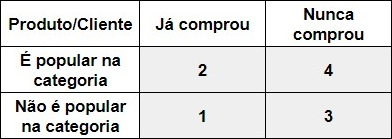
\includegraphics[width=12cm]{doc/latex/text/images/fc-categ.jpg}
    \caption{Avaliação FC geral ou por categoria.}
    \label{fig:fc-categ}
\end{figure}

\begin{figure}[htp]
    \centering
    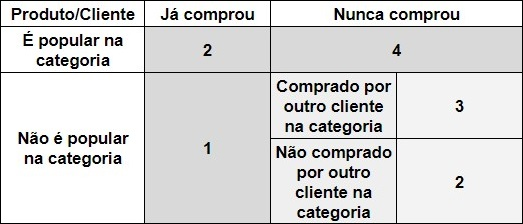
\includegraphics[width=12cm]{doc/latex/text/images/fc-intercateg.jpg}
    \caption{Avaliação FC por intercategorias}
    \label{fig:fc-intercateg}
\end{figure}

Tendo os métodos de avaliação definidos, sua lógica foi descrita em \textit{scripts} Python. Cada \textit{script} contém instruções para percorrer todos os registros em cada um dos \textit{datasets} selecionados, analisar os produtos mais vendidos de acordo com uma categorização de cliente e produzirem um \textit{dataset} de saída contendo 3 colunas: código do cliente, código do produto e avaliação.

No caso dos \textit{datasets} provenientes do repositório UCI ML, decidiu-se categorizar os clientes com base na coluna \textit{country} (país de origem). No caso do conjunto do Kaggle, que aborda transações exclusivamente realizadas no Brasil, a coluna \textit{customer\_state} (UF de origem) serviu de base para categorização de clientes.

Após terem sido produzidas avaliações para os 3 \textit{datasets} selecionados, esses valores foram analisados sob o ponto de vista da estatística descritiva, de forma a entender como cada método avaliou os dados contidos no dataset. O resultados dessa análise serão explicados em mais detalhes na Seção \ref{resultados}.

\section{Geração de recomendações} \label{geracao-rec}
Após a geração de avaliações conforme os métodos definidos na Seção \ref{definicao-crit}, os \textit{datasets} resultantes foram utilizados como entrada para o treinamento da rede neural descrita por Tanner. A rede consiste em 4 camadas iniciais, que fazem o processo de \textit{embedding} dos produtos e clientes, e 3 camadas do tipo Dense, que permitem à rede relacionar as entradas categóricas com as avaliações durante o treinamento.

\begin{figure}[htp]
    \centering
    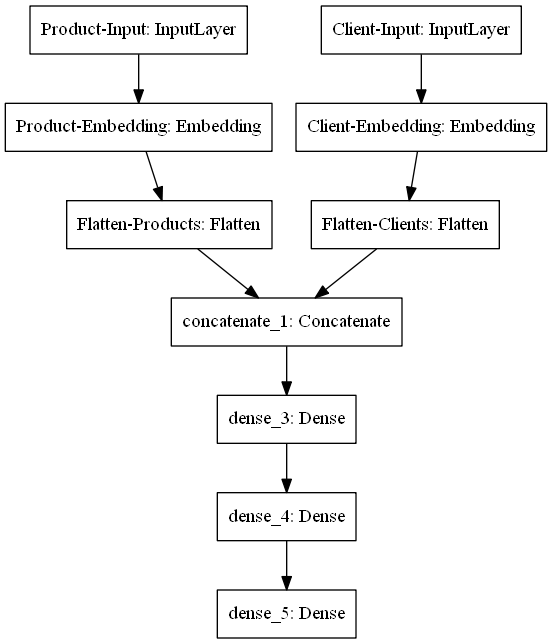
\includegraphics[width=10cm]{doc/latex/text/images/network.png}
    \caption{Estrutura de rede neural utilizada}
    \label{fig:fc-intercateg}
\end{figure}

Essa estrutura de rede foi escolhida para o trabalho pois apresenta as seguintes vantagens:

\begin{itemize}
    \item Conforme detalhado na Seção \ref{sist-rec}, o uso de \textit{embeddings} em \textit{Machine Learning} permite a redução de dimensionalidade e por consequência uma melhor utilização de recursos computacionais tais como memória RAM e processamento
    \item Consolida o processo de criação e aprendizado do \textit{embedding} na mesma estrutura, facilitando o entendimento e manutenção do código.
    \item O funcionamento da estrutura foi documentado pelo autor tanto em texto quanto em vídeo, o que permite entendê-lo e comprová-lo de forma mais assertiva.
\end{itemize}

A rede neural foi treinada utilizando um \textit{dataset} de entrada de cada vez. Após o treinamento, a rede foi testada manualmente com pares de produtos/clientes do \textit{dataset} para atestar que o treinamento ocorreu de forma bem sucedida.